\documentclass[twocolumn]{aastex61}
%\documentclass{emulateapj}
%\usepackage[colorlinks,urlcolor=blue,citecolor=blue,linkcolor=blue]{hyperref} 
\usepackage{graphicx,natbib}
\citestyle{aa}
\usepackage[space]{grffile}
\usepackage{latexsym}
\usepackage{amsfonts,amsmath,amssymb}
\usepackage{url}
\usepackage[utf8]{inputenc}
\usepackage{fancyref}
\usepackage{hyperref}
\usepackage{multirow}
\hypersetup{colorlinks=false,pdfborder={0 0 0},}

\newcommand{\rf}{\emph{realfast}}
\newcommand{\frb}{FRB 121102}

\begin{document}

\title{The \frb\ Campaign, a Multi-Telescope Burst Detection, and Implications for the FRB Population}
\shorttitle{\frb\ Observing Campaign}
\shortauthors{Law et al.}

\author[0000-0002-4119-9963]{C.~J.~Law}
\affiliation{Department of Astronomy and Radio Astronomy Lab, University of California, Berkeley, CA 94720, USA}

\author{C.~G.~Bassa}
\affiliation{ASTRON, Netherlands Institute for Radio Astronomy, Postbus 2, 7990 AA, Dwingeloo, The Netherlands}

\author{G.~C.~Bower}
\affiliation{Academia Sinica Institute of Astronomy and Astrophysics, 645 N. A'ohoku Place, Hilo, HI 96720, USA}

\author{S.~Burke-Spolaor}
\affiliation{National Radio Astronomy Observatory, Socorro, NM 87801, USA}
\affiliation{Department of Physics and Astronomy, West Virginia University, Morgantown, WV 26506, USA}
\affiliation{Center for Gravitational Waves and Cosmology, West Virginia University, Chestnut Ridge Research Building, Morgantown, WV 26505}

\author{B.~J.~Butler}
\affiliation{National Radio Astronomy Observatory, Socorro, NM 87801, USA}

\author{T.~Cantwell}
\affiliation{Jodrell Bank Centre for Astrophysics, Alan Turing Building, School of Physics \& Astronomy ,The University of Manchester, Oxford Road, Manchester M13 9PL, UK}

\author{S.~H.~Carey}
\affiliation{Astrophysics Group, Cavendish Laboratory, 19 J. J. Thomson Avenue, Cambridge CB3 0HE, UK}

\author{S.~Chatterjee}
\affiliation{Cornell Center for Astrophysics and Planetary Science and Department of Astronomy, Cornell University, Ithaca, NY 14853, USA}

\author{J.~M.~Cordes}
\affiliation{Cornell Center for Astrophysics and Planetary Science and Department of Astronomy, Cornell University, Ithaca, NY 14853, USA}

\author{P.~Demorest}
\affiliation{National Radio Astronomy Observatory, Socorro, NM 87801, USA}

\author{R.~Fender}
\affiliation{Centre for Astrophysical Surveys, University of Oxford, Denys Wilkinson Building, Keble Road, Oxford OX1 3RH, UK}

\author{K.~Grainge}
\affiliation{Jodrell Bank Centre for Astrophysics, Alan Turing Building, School of Physics \& Astronomy ,The University of Manchester, Oxford Road, Manchester M13 9PL, UK}

\author{J.~W.~T.~Hessels}
\affiliation{ASTRON, Netherlands Institute for Radio Astronomy, Postbus 2, 7990 AA, Dwingeloo, The Netherlands}
\affiliation{Anton Pannekoek Institute for Astronomy, University of Amsterdam, Science Park 904, 1098 XH Amsterdam, The Netherlands}

\author{J.~Hickish}
\affiliation{Dept of Astronomy and Radio Astronomy Lab, University of California, Berkeley, CA 94720, USA}
\affiliation{Astrophysics Group, Cavendish Laboratory, 19 J. J. Thomson Avenue, Cambridge CB3 0HE, UK}

\author{V.~M.~Kaspi}
\affiliation{Department of Physics and McGill Space Institute, McGill University, 3600 University St., Montreal, QC H3A 2T8, Canada}

\author{T.~J.~W.~Lazio}
\affiliation{Jet Propulsion Laboratory, California Institute of Technology, Pasadena, CA 91109, USA}

\author{M.~A.~McLaughlin}
\affiliation{Department of Physics and Astronomy, West Virginia University, Morgantown, WV 26506, USA}
\affiliation{Center for Gravitational Waves and Cosmology, West Virginia University, Chestnut Ridge Research Building, Morgantown, WV 26505}

\author{D.~Michilli}
\affiliation{ASTRON, Netherlands Institute for Radio Astronomy, Postbus 2, 7990 AA, Dwingeloo, The Netherlands}
\affiliation{Anton Pannekoek Institute for Astronomy, University of Amsterdam, Science Park 904, 1098 XH Amsterdam, The Netherlands}

\author{K.~Mooley}
\affiliation{Centre for Astrophysical Surveys, University of Oxford, Denys Wilkinson Building, Keble Road, Oxford OX1 3RH, UK}

\author{Y.~C.~Perrott}
\affiliation{Astrophysics Group, Cavendish Laboratory, 19 J. J. Thomson Avenue, Cambridge CB3 0HE, UK}

\author{S.~M.~Ransom}
\affiliation{National Radio Astronomy Observatory, Charlottesville, VA 22903, USA}

\author{N.~Razavi-Ghods}
\affiliation{Astrophysics Group, Cavendish Laboratory, 19 J. J. Thomson Avenue, Cambridge CB3 0HE, UK}

\author{M.~Rupen}
\affiliation{National Research Council of Canada, Herzberg Astronomy and Astrophysics, Dominion Radio Astrophysical Observatory, P.O. Box 248, Penticton, BC V2A 6J9, Canada}

\author{A.~Scaife}
\affiliation{Jodrell Bank Centre for Astrophysics, Alan Turing Building, School of Physics \& Astronomy ,The University of Manchester, Oxford Road, Manchester M13 9PL, UK}

\author{P.~Scott}
\affiliation{Astrophysics Group, Cavendish Laboratory, 19 J. J. Thomson Avenue, Cambridge CB3 0HE, UK}

\author{P.~Scholz}
\affiliation{National Research Council of Canada, Herzberg Astronomy and Astrophysics, Dominion Radio Astrophysical Observatory, P.O. Box 248, Penticton, BC V2A 6J9, Canada}

\author{A.~Seymour}
\affiliation{Arecibo Observatory, HC3 Box 53995, Arecibo, PR 00612, USA}
\affiliation{Max-Planck-Institut f\"ur Radioastronomie, Auf dem H\"ugel 69, D-53121 Bonn, Germany}

\author{L.~G.~Spitler}
\affiliation{Max-Planck-Institut f\"ur Radioastronomie, Auf dem H\"ugel 69, D-53121 Bonn, Germany}

\author{S.~P.~Tendulkar}
\affiliation{Department of Physics and McGill Space Institute, McGill University, 3600 University St., Montreal, QC H3A 2T8, Canada}

\author{D.~Titterington}
\affiliation{Astrophysics Group, Cavendish Laboratory, 19 J. J. Thomson Avenue, Cambridge CB3 0HE, UK}

\author{R.~S.~Wharton}
\affiliation{Cornell Center for Astrophysics and Planetary Science and Department of Astronomy, Cornell University, Ithaca, NY 14853, USA}

\author{P.~K.~G.~Williams}
\affiliation{Harvard-Smithsonian Center for Astrophysics, Cambridge, MA, USA}

\begin{abstract}
We present results of the coordinated observing campaign that made the first localization of a Fast Radio Burst, FRB 121102. Of the nine bursts detected by the Very Large Array at 3~GHz, three had simultaneous observing coverage at other observatories, of which one was detected by the Arecibo Observatory at 1.4~GHz. We use multi-observatory detection and constraints with modeling of bursts only seen at 3~GHz to show that burst spectra are not well characterized by a powerlaw. Instead, bursts typically have a $\sim500$~MHz-scale envelope in which the apparent radio energy emitted is as high as $10^{40}$\ erg. The dispersion measure apparently changes significantly between bursts, which suggests that they have intrinsic spectral structure that can bias the estimate of DM by as much as 5 pc cm$^{-3}$. We use \frb\ as a prototype of the FRB class to estimate a volumetric rate of $R_{\rm{FRB}} \approx 5\times10^{-5}$\ Mpc$^{-3}$\ yr$^{-1}$ for the cosmic volume out to redshift of 1. This rate is broadly consistent with models of FRBs from young magnetars or fast pulsars, if the typical FRB repeats on the order of $10^3$\ times in its life.
\end{abstract}

\section{Introduction}

Fast Radio Bursts (FRBs) were discovered ten years ago as a millisecond-duration radio transient with an anomalously high dispersion measure \citep[the ``Lorimer burst'';][]{2007Sci...318..777L}. Their large dispersion measures (DM) implied that they originated outside of our Galaxy, potentially at cosmological distances, and were orders of magnitude more luminous than any other millisecond radio transient \citep{2013Sci...341...53T}. Both their energetics and distance have inspired a wide variety of models and astrophysical applications \citep[e.g.,][]{2014ApJ...780L..33M, 2014ApJ...797...70K, 2016MNRAS.458L..19C, 2016MNRAS.457..232C}. However, that potential was limited by the lack of a definitive association of an FRB to an extragalactic host.

This paper is part of a series based on the first localization of an FRB and its unambiguous association to an extragalactic host \citep{LOC, OPT, EVN}. \frb, also known as the ``repeating FRB'', was first detected in November 2012 by the Arecibo Observatory \citep{2014ApJ...790..101S}. In mid 2015, new Arecibo observations revealed a series of bursts at the same DM ($\sim559$\ pc cm$^{-3}$) and sky position that rules out cataclymic models for this source \citep{2016Natur.531..202S}. Beginning in August of 2015, we made the first of nine detections of \frb\ with the Very Large Array \citep{LOC} and localized it with a precision of 0.1\arcsec. Subsequent radio and optical observing discovered more bursts from \frb\ and associated them with a persistent radio and optical source at a redshift of 0.193 with a precision of 0.01\arcsec \citep[$\sim40$\ pc]{OPT, EVN}.

\frb\ has now been localized four orders of magnitude better than any other FRB and placed at a cosmological distance. Its lookback and luminosity distances are 746 and 972 Mpc, assuming a concordance cosmology with parameters given by \citet{2016A&A...594A..13P}. This association means that \frb\ is orders of magnitude more luminous than any other millisecond transient and that its DM traces both the host and intergalactic medium \citep{OPT}. If \frb\ is representative of all FRBs, then we should expect them to be useful as probes of the intergalactic medium and their host galaxies. Thus, the confirmation of a cosmological distance for \frb\ has begun to fulfil the promise implied by the Lorimer burst.

Although new models of FRB origin have been already been developed \citep{2017arXiv170104815K, 2017arXiv170102370M, 2017arXiv170104094Z, 2017arXiv170102492D}, we still do not know what causes them. Its coincidence with a compact, persistent radio source is consistent with \frb\ as a young magnetar powering a luminous pulsar wind nebula \citep{2017arXiv170104815K}. At the same time, \frb\ is found in a low-metallicity dwarf galaxy, which is the preferred environment for long GRBs and Type-I superluminous supernovae \citep[LGRB and SLSN-I, respectively;][]{2017arXiv170102370M}. It has been suggested that these other classes of transient are signatures of the birth of magnetars that are only born in low-metallicity environments \citep{2014ApJ...787..138L}.

%Also, it has not been demonstrated that \frb\ is representative of the overall FRB population. In fact, the repetition of its bursts is unique among all FRBs \citep{2015MNRAS.454..457P}, so it is natural to ask whether \frb\ is representative. An important first step is to demonstrate that the properties of \frb\ are consistent with the significant body of facts for the overall population \citep{2015MNRAS.451.3278M, 2016MPLA...3130013K}. The repeating nature of \frb\ provides us with a sample of bursts covering a range of spectral properties, temporal properties, and luminosities that can be used to test its connection to the larger FRB population.

If we assume that \frb\ is representative of all FRBs, we use it to constrain the physical processes at play in the overall FRB population. We know that FRBs are extremely energetic, more data is needed to determine if that traces intrinsic processes, such as coherent, pulsar-like emission \citep{2014PhRvD..89j3009K, 2014ApJ...785L..26L, 2016MNRAS.457..232C} or if extrinsic effect also play a role \citep{2015MNRAS.451.3278M, CORDES}. The paper presents an analysis of the spectral properties of VLA bursts implied by simultaneous observing at Effelsberg, GBT, AMI-LA, and Arecibo, including the first simultaneous detection of an FRB at two observatories. The repetition of \frb\ also has strong implications for calculations of their rate of occurrence \citep{2016MNRAS.458L..89C} and comparison to other classes of transient, such as superluminous supernovae \citep{OPT}.

In Section \ref{sec:obs}, we describe the multi-telescope observing campaign and a refined analysis of the nine VLA bursts. Section \ref{sec:res} presents the first spectrum of an FRB simultaneously detected at multiple telescopes and show that burst spectra cannot be modeled with a single spectral index. We then model the dynamic spectra to characterize the burst spectra, energies, and dispersion properties.
\ref{sec:disc} discusses implications of the properties of \frb\ bursts on inferences about the overall FRB population, including an estimate of the FRB volumetric rate. Finally, we close with a discussion of how the \frb\ burst spectra, host properties, burst rate estimates, and other properties inform new strategies for finding FRBs.

\section{Observations}
\label{sec:obs}
\begin{figure*}[t]
\begin{center}
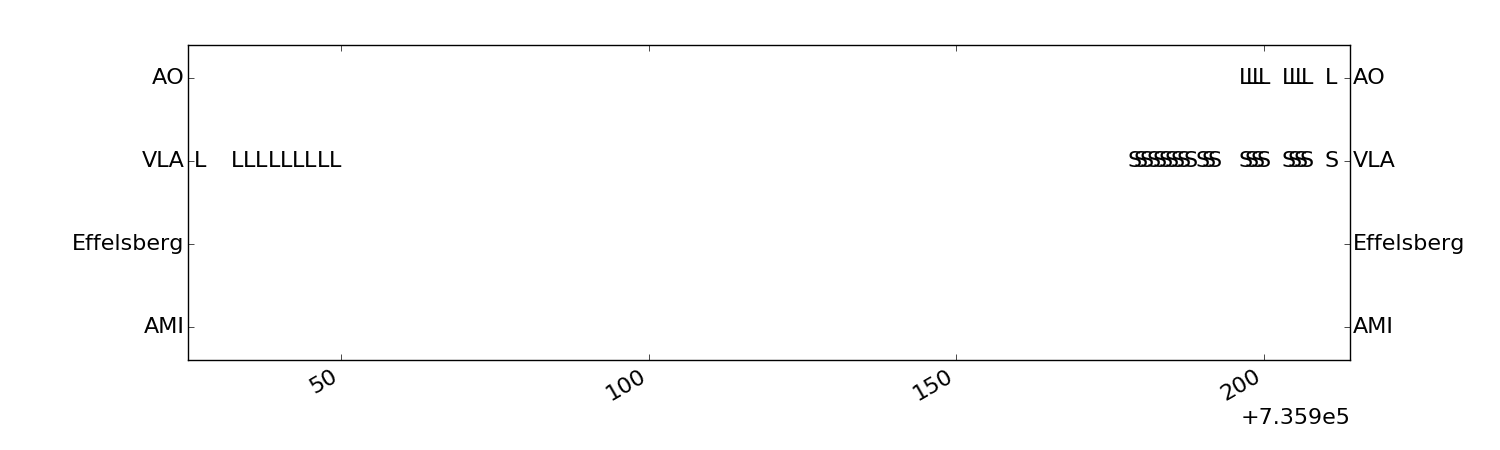
\includegraphics[width=2\columnwidth]{timeline0}

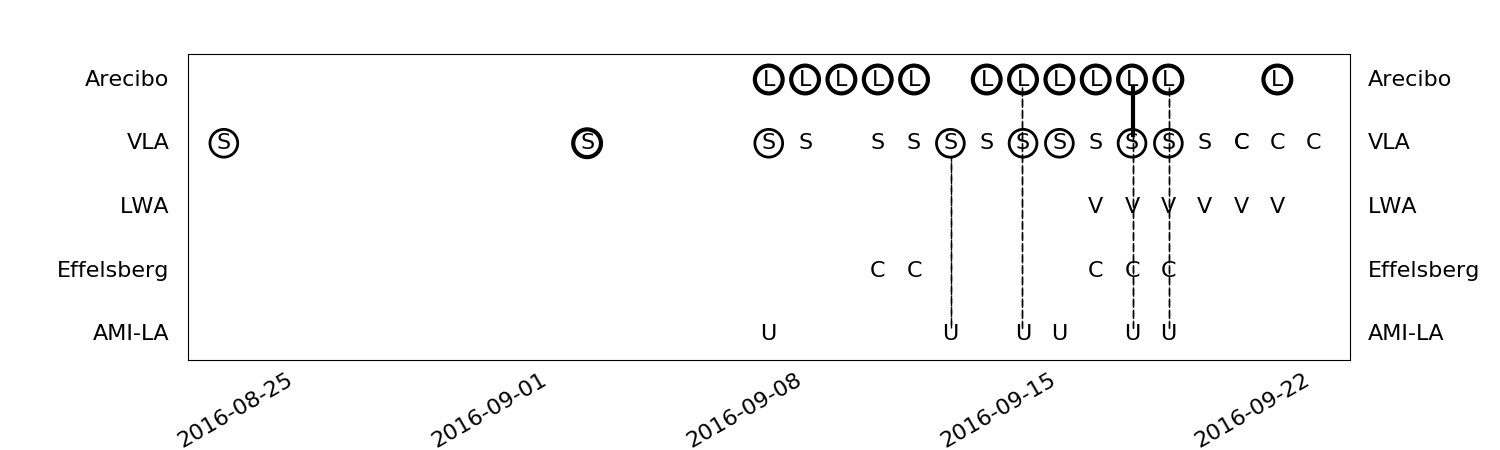
\includegraphics[width=2\columnwidth]{timeline}
\caption{The top and bottom panels summarize the observing coverage and detections of \frb\ in the 2015 and 2016 campaigns. Symbols show days with observations with letters L, S, C, K referring to radio frequencies of 1.4, 3, 4.5, and 12~GHz, respectively. Circles highlight observations that detected bursts from \frb. Multiple circles indicate multiple burst detections, except for Arecibo, which typically has multiple detections per observing session. The black dashed lines show the VLA burst detections with simultaneous coverage at other telescopes. The solid black line shows the simultaneous burst detection at VLA and Arecibo.
\label{fig:sched}}
\end{center}
\end{figure*}

The data presented here were obtained from multiple programs and telescopes with a goal of interferometrically localizing \frb\ with the VLA. We coordinated observing between the VLA, Arecibo, Effelsberg, and AMI-LA telescopes, as shown in Figure \ref{fig:sched}. Below, we summarize these observations, with a focus on those conducted simultaneously with VLA burst detections from \frb.

\subsection{VLA}

The \frb\ observing campaign started in late 2015 with a 10~hr campaign ($\sim1$~hr per session) observed at 1.4~GHz in the compact D configuration. In April through May 2016, we conducted a 40~hr campaign ($\sim2$~hr per session) at 3~GHz in the C and CnB configurations in coordination with Arecibo \citep{2016arXiv160308880S}. We concluded with a 40~hr, coordinated campaign ($\sim2$~hr per session) from August through September 2016 in the B configuration and during the move to the most extended A configuration. In the late-2016 campaign, the first 34 hours of VLA observations were made at 3~GHz, while the last 6 hours were observed at 6~GHz. This paper focuses on the data collected at 3~GHz, which includes all nine burst detections and is the widest bandwidth to have ever detected an FRB.

All VLA fast-sampled data were observed with 5~ms sampling, 256 channels, and dual-circular polarization \citep{2015ApJ...807...16L}. The channel frequency width was set to maximize sensitivity to the known DM of \frb\ with the largest total bandwidth. The total bandwidth at L (1.4~GHz), S (3~GHz), and C (6~GHz) bands was 256~MHz, 1024~MHz, and 2048~MHz, respectively. The 3~GHz data were recorded data in eight spectral windows with 32 channels each.

Observations in August and September were searched by a prototype version of \rf\footnote{See \url{http://realfast.io}.}. \rf\ is a real-time, fast imaging transient search system. The current prototype runs on CPU-based hardware that is normally dedicated to the VLA correlator; for this experiment, it runs the transient search pipeline software called \emph{rtpipe} \citep[\url{https://github.com/caseyjlaw/rtpipe};][]{2015ApJ...807...16L}. Images were formed for each integration with a DM grid of 0, 546, 556.9, 560, and 565 pc cm$^{-3}$ and a time resampling grid of 5, 10, 20, 40, and 80 ms. This DM grid was chosen to maintain 90\% sensitivity to the nominal DM range of 540--570 pc cm$^{-3}$, which includes the known \frb\ DM of 559 pc cm$^{-3}$ \citep{2016arXiv160308880S}. Gain calibration was made from observations of J0555+3948 by the telcal system, which uses phase-only calibration. A flux scale is calculated for each spectral window from an observation of 3C48 and applied to all burst spectra.

Burst detections and localizations were made within hours of data being recorded. The transient search starts when data are recorded and proceeds slower than real-time, so we refer to it as ``quasi real-time''. For each trial DM, integration, and time scale, we form an image and calculate the S/N ratio for the peak pixel in the dirty image. We empirically identified S/N thresholds of 6.4 and 7.4 as useful to capture data quality statistics and candidates for inspection, respectively. The higher threshold is relatively unlikely to be triggered by thermal noise in this configuration, so \rf\ generates a more detailed (and computationally intensive) candidate visualization that includes an image and spectrum. All visibilities are recorded so detailed analysis, including improved calibration and localization, can be conducted offline. 

Computational (Jupyter) notebooks to reproduce the transient detection, localization, and analysis presented here can be found at \url{https://github.com/caseyjlaw/FRB121102}. Time cut-out visibility data and calibration products are available at \url{https://doi.org/10.7910/DVN/TLDKXG}. Original visibility data are available under VLA program codes 16A-459 and 16A-496 and can be downloaded at \url{http://archive.nrao.edu}.

\subsection{Arecibo}

During the late-2016 campaign, Arecibo observed with the L-wide receiver using the PUPPI pulsar backend. The observational frequency range was 1.15 to 1.73~GHz and frequency resolution was 1.5625~MHz, which has a typical sensitivity of 2~mJy in 2~ms ($1\sigma$). We recorded total full Stokes polarization intensity spectra with a time resolution of 10.24~$\mu$s. Each frequency channel was coherently dedispersed to 557~pc cm$^{-3}$, thereby eliminating intra-channel dispersion smearing. The full width at half maximum (FWHM) beam size at band center is 3.3\arcmin.

In total, 11 Arecibo observations had some simultaneous coverage with the VLA. All of these observations were conducted while pointing at the location of \frb\ measured by the VLA. Three of those observations had simultaneous coverage of VLA bursts and one of those Arecibo observations detected the VLA burst. 
% During the first VLA burst with Arecibo coverage (MJD 57643), the PUPPI 1.4~GHz recording system failed so data were recorded at C band with the mock spectrometer. The C-band observations were recorded at frequencies from 4078 to 4245~MHz and had a sensitivity of 3.6~mJy in 2~ms ($1\sigma$). No detection was made in those Arecibo data. % levels set wrong. useless c-band ao data.
Overall, there were many more bursts detected at Arecibo than with the VLA and a more detailed analysis of those bursts will be presented elsewhere (Michilli et al, in prep).

\subsection{Effelsberg}

Effelsberg observations were conducted with the S60mm receiver at an observing frequency of 4.6 to 5.1~GHz. Total intensity spectra were recorded by the PFFTS backend in pulsar search mode with a time resolution of 65.5~$\mu$s and 128 frequency channels. The receiver has a system equivalent flux density is 18 Jy and a FWHM beam size of 2.4\arcmin\ at 4.85~GHz. 

Five Effelsberg observations were made pointing at the known location of \frb\ and had some simultaneous coverage with the VLA; two observations were simultaneous with VLA bursts. Unfortunately, due to a configuration error, a 100~MHz bandwidth filter centered at 4.85~GHz was in place for both of these sessions. The sensitivity was about 28 mJy in 2 ms ($1\sigma$), which is two times worse than the nominal value. No burst was detected in either observation.

\subsection{AMI-LA}

We observed \frb\ with the Arcminute MicroKelvin Imager Large Array (AMI-LA; Zwart et al. 2008) for 3 hours each on four epochs starting at MJDs 57643, 57645, 57648, and 57649. Observations were made with the new digital correlator having 4096 channels across a 5~GHz bandwidth between 13--18~GHz with a 1~s integration time. The phase calibrator, J0518+3306, was observed every 12 minutes for about 1.5 minutes. The AMI-LA data were binned to eight 0.625~GHz channels and processed (RFI excision and calibration) with a fully-automated pipeline, AMI-REDUCE \citep[e.g.,][]{2013MNRAS.429.3330P}. Daily measurements of 3C48 and 3C286 were used for the absolute flux calibration, which is good to about 10\%. 

We inspected the calibrated visibilities, and did not find any signal above 30 mJy in the 1s samples at and in the vicinity of the detected bursts. Concatenating and imaging the 12 hours of calibrated data with the CASA tasks {\it concat} and {\it clean} also does not yield any significant detection at the FRB location. Although the statistical $3\sigma$\ upper limit is 60 $\mu$Jy, extended mJy-level sources in the field cause sidelobe confusion (the AMI-LA angular resolution is $\sim$30\arcsec), and the actual upper limit is larger. We introduced artificial point sources at the FRB location using the CASA {\it sm} tool, and found that these sources can be recovered as long as their peak flux densities are more than $\sim100\mu$Jy. Hence, we place an upper limit of $100\pm10 \mu$Jy on any quiescent or possible radio flaring on $\sim$days timescales from the FRB. This limit is similar to the flux density measured by the VLA \citep{LOC}.

\section{Results}
\label{sec:res}

\subsection{Multi-Observatory Burst Spectrum}

Four of the VLA bursts were observed simultaneously with either Arecibo, Effelsberg, or AMI-LA, and two were observed simultaneously with all four observatories (Figure \ref{fig:sched}). Of these bursts, only one VLA burst (on 17 Sep 2016) was simultaneously detected by another observatory (Arecibo). 

Figure \ref{fig:sgram} shows a dynamic spectrum for this burst with both VLA and AO data. The temporal resolution of the VLA data (5~ms) is much coarser than that of Arecibo, so data were resampled to the same temporal grid after correcting for barycentric and dispersion measure offsets. The dispersion correction for both data sets assumed a DM of 560.5 pc cm$^{-3}$, which was typical of the source during the observing campaign \citep{WEIRD}. The regridded dynamic spectrum has an apparent DM error that is evident both as a frequency-dependent time drift within the Arecibo observation and as an offset between the Arecibo and VLA bursts. Both of these drifts are consistent with an apparent DM of $\sim$565 pc cm$^{-3}$. This is consistent with modeling of the VLA spectrum described in \S \ref{sec:spec}.

Figure \ref{fig:multi} shows spectra built from integrated flux densities measured (or limited) during three burst with multi-telescope observing coverage. The burst on 17 Sep 2016 was detected with Arecibo and the VLA with significances of 25$\sigma$\ and 39$\sigma$\ with integrated flux densities of 111 mJy and 14 mJy, respectively. Assuming a powerlaw flux density model ($S_{\nu} \propto \nu^{\alpha}$), we find a spectral index $\alpha=2.7$. This is inconsistent with the spectral index limit implied by the Effelsberg nondetection at 4.5~GHz ($\alpha<0.6$\ for a 2~ms burst and $5\sigma$ limit).

Overall, the bursts with simultaneous observing coverage are not consistent with a powerlaw model for the burst spectra. Two Arecibo nondetections and two Effelsberg nondetections of VLA bursts place mutually inconsistent lower and upper limits on the spectral index. The Arecibo upper limits at 1.4~GHz imply that burst spectral indices $\alpha_{1.4/3}>+3.7$, while at Effelsberg the flux limits require $\alpha_{3/4.5}<-0.4$. The strictest limits on $\alpha_{1.4/3}$\ and $\alpha_{3/4.5}$\ are both derived from the burst on 18 Sep 2016, which shows that a powerlaw model is inappropriate even for a single burst.

\begin{figure}[htb]
\begin{center}
 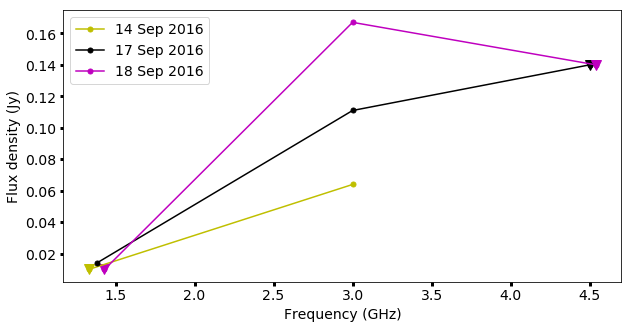
\includegraphics[width=\columnwidth]{multispec.png}
 \caption{Broadband spectra for three bursts of \frb\ with simultaneous multi-telescope observing coverage. Measurements are shown with dots and upper limits with triangles. Upper limits assume a pulse width of 2~ms and a $5\sigma$ detection threshold. Overlapping points are offset by a few tens of MHz in frequency for visualization.
 \label{fig:multi}}
\end{center}
\end{figure}

\subsection{VLA Bursts}

\begin{figure*}[htb]
\begin{center}
 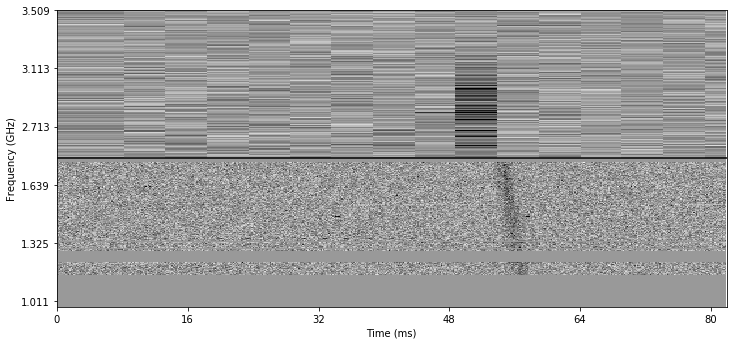
\includegraphics[width=1.9\columnwidth]{aovla_spec.png}
 \caption{Composite dynamic specrum for the burst from \frb\ on MJD 57648 with data from the VLA and Arecibo observatories. Both data sets have been barycentered and corrected for an assumed dispersion measure of 560.5 pc $^{-3}$. The black line separates data from the VLA (2.5 to 3.5~GHz) and Arecibo (1.0 to 1.8~GHz). The amplitude scale is normalized by assuming the Arecibo to VLA gain ratio is 10.
 \label{fig:sgram}}
\end{center}
\end{figure*}

\subsubsection{Spectral Modeling}
\label{sec:spec}

This paper refines the analysis of the nine VLA radio burst spectra described in \citet{LOC} in a few ways. We use a better calibration scheme and have optimized the detection significance over a fine grid of DM ($\Delta \rm{DM}=1\ \rm{pc}\ \rm{cm}^{-3}$). After calibration and flagging, the visibility phases were rotated to the best-fit location \citep[(RA, Dec) $=$ (05h31m58.70s, +33d08m52.5s);][]{LOC} to extract a Stokes I spectrum that maximizes the image S/N for each burst.

Table \ref{tab:spec} summarizes the properties of all nine VLA bursts. Parameters such as integrated flux density, S/N, and Stokes V were measured from the burst properties integrated in frequency. Stokes V values estimated from the dual-circular feeds ($(RR-LL)/(RR+LL)\approx3\%$ and are comparble to the systematic error expected from the primary beam (Perley et al 2016, VLA memo). Given that systematic effects dominate the apparent circular polarization, this observation limits the fractional circular polarization is less than 3\%.

\begin{table*}
\caption{Properties of Bursts from \frb}
\centering
\begin{tabular}{cc|ccc|cccccc}
\multicolumn{2}{c|}{Time} & \multicolumn{3}{c|}{Observered properties} & \multicolumn{6}{c}{Modeled properties} \\ \hline
Calendar day & Burst time   & Image S/N & S$_{\rm{I,int}}$	& S$_{\rm{V}}$ 	& DM$_{\rm{opt}}$ 	& dt 			& S$_{\rm{I,peak}}$ & Center & FWHM & E$_{\rm{int}}$ \\
(2016)       &  (MJD)     &           & (mJy) 			& (mJy) 		& (pc cm$^{-3})$ 	& (ms) 			& (mJy) 			& (GHz)  & (MHz) & ($10^{38}$\ erg)\\ \hline
23 Aug & 57623.74402686      & 38 		& 194				& +3			& 567$\pm2$ 		& 2.0$\pm0.2$	 		& 690 		& 2.8 		& 290 & 11 			\\
2 Sep & 57633.67986367      & 179 		& 1500				& --35 			& 568.2$\pm0.2$ 	& 2.05$\pm0.02$			& 3340 		& 3.2 		& 510 & 98				\\
2 Sep\tablenotemark{a} & 57633.69515938 & 15 & 69			& +2			& 562$^{+4}_{-6}$ 	& 2.5$^{+0.9}_{-0.6}$	& $>$430 	& $<$2.5	& 290 & 7  			\\
7 Sep & 57638.49937435      & 12 		& 55				& +5 			& 567$^{+7}_{-9}$ 	& 1.3$^{+1.4}_{-0.8}$	& 130 		& 3.1 		& 420 & 3  			\\
12 Sep & 57643.45730263      & 100 		& 508				& --5 			& 565.6$^{+0.6}_{-0.5}$ & 1.9$\pm0.1$		& 1170 		& 2.8 		& 510 & 34 			\\
14 Sep & 57645.42958602      & 13 		& 64 				& +3			& 563$^{+5}_{-4}$ 	& 1.0$\pm0.7$		 	& 170 		& 2.8 		& 380 & 4  			\\
15 Sep\tablenotemark{a} & 57646.46600650 & 20 & 87			& +1			& 569$\pm5$ 		& 2.7$^{+0.9}_{-1.4}$	& $>$420 	& $<$2.5 	& 430 & 10 			\\
17 Sep\tablenotemark{b} & 57648.43691490 & 25 & 111			& +9			& 564$\pm2$ 		& 1.4$^{+0.3}_{-0.4}$	& 260 		& 2.8 		& 470 & 7  			\\
18 Sep & 57649.45175697      & 36 		& 167				& +1			& 567$\pm2$ 		& 2.1$\pm0.5$		 	& 290 		& 3.0 		& 690 & 12 			\\ \hline
\end{tabular}
\tablenotetext{a}{Best-fit Gaussian is not centered in 3~GHz band, so spectral parameters are limits.}
\tablenotetext{b}{Detected simultaneously with Arecibo between 1.15 and 1.73~GHz.}
\label{tab:spec}
\end{table*} 

Figure \ref{fig:spec} shows that the Stokes I spectra are generally characterized by a broad, Gaussian shape with inter-channel modulation as high as 100\%. To better understand the spectra, we extracted dynamic radio spectra (time versus frequency) for 2d modeling with the MCMC sampler \emph{emcee} \citep{2013PASP..125..306F}. MCMC sampling requires a generative model for the data, so we wrote functions in Python to create 2d dynamic spectra. The dynamic spectra are generated in the spectral domain as a Gaussian envelope (with amplitude, center, and width) and in the temporal domain by a start time, temporal width, and DM. We assume a dispersive delay that scales as frequency squared.

The 6-dimensional models were sampled with 100 walkers taking 500 steps. Typically, the first 200 steps were used to burn in the walkers and were ignored. A flat prior was used over all ranges with valid data. An additional requirement was that the integrated burst signal must have a detection significance higher than 8$\sigma$. The inter-channel modulation (scintillation) was ignored in the model. The measured, off-burst noise value was typically 70 mJy per 5~ms integration and 4~MHz channel.

The parameters for the best model of the dynamic spectrum are given in Table \ref{tab:spec} and the resulting Gaussian model overlaid on Figure \ref{fig:spec}. The typical burst has a spectral width of 500~MHz. All but two of the best-fit Gaussians are centered inside the 3~GHz band and some appear contained by the 1~GHz wide band. This is consistent with previous detections of \frb\ by Arecibo, which showed quasi-broadband structure \citep{2016arXiv160308880S} and large variation in the implied spectral index \citep{2014ApJ...790..101S}. 

\begin{figure*}[ht]
\begin{center}
 \begin{minipage}{2\columnwidth}
  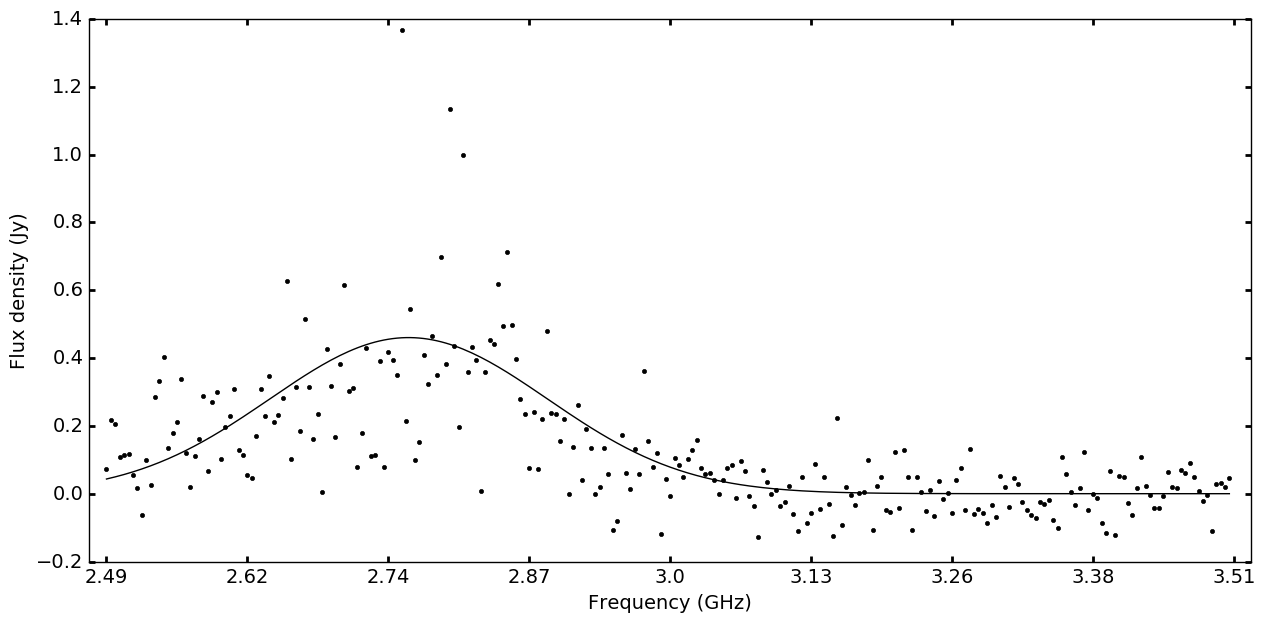
\includegraphics[width=0.33\columnwidth]{spec_57623.png}
  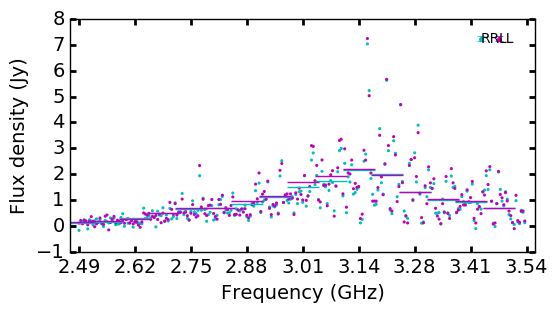
\includegraphics[width=0.33\columnwidth]{spec_57633_scan7.png}
  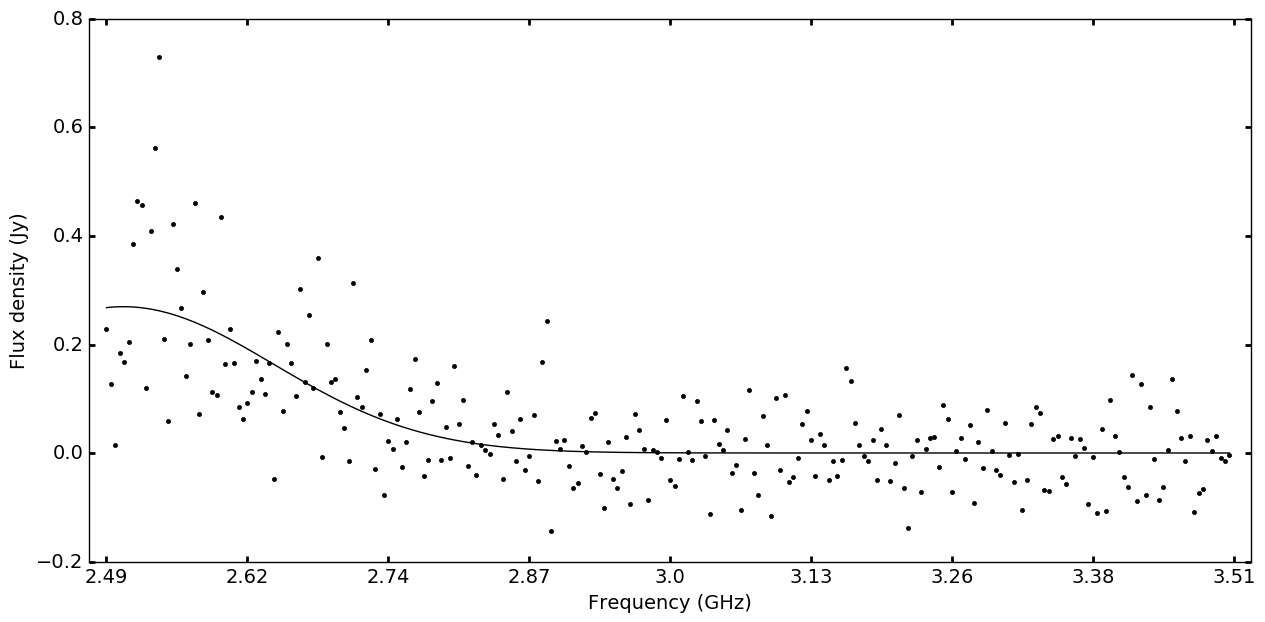
\includegraphics[width=0.33\columnwidth]{spec_57633_scan13.png}
 \end{minipage}

 \begin{minipage}{2\columnwidth}
  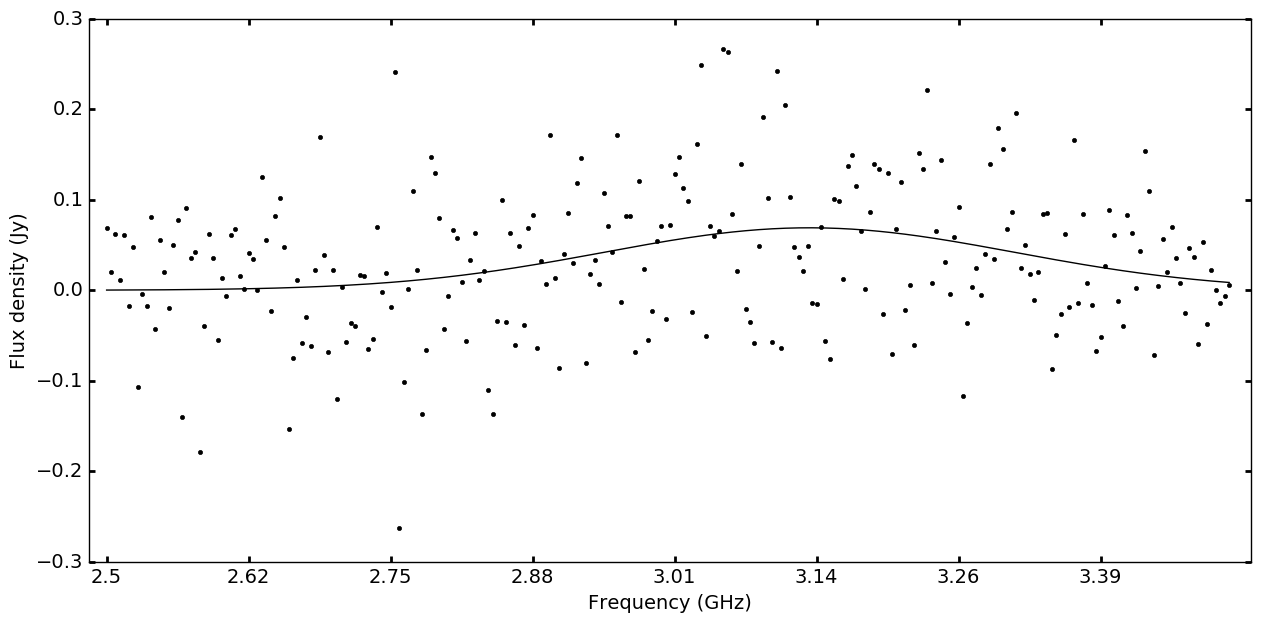
\includegraphics[width=0.33\columnwidth]{spec_57638.png}
  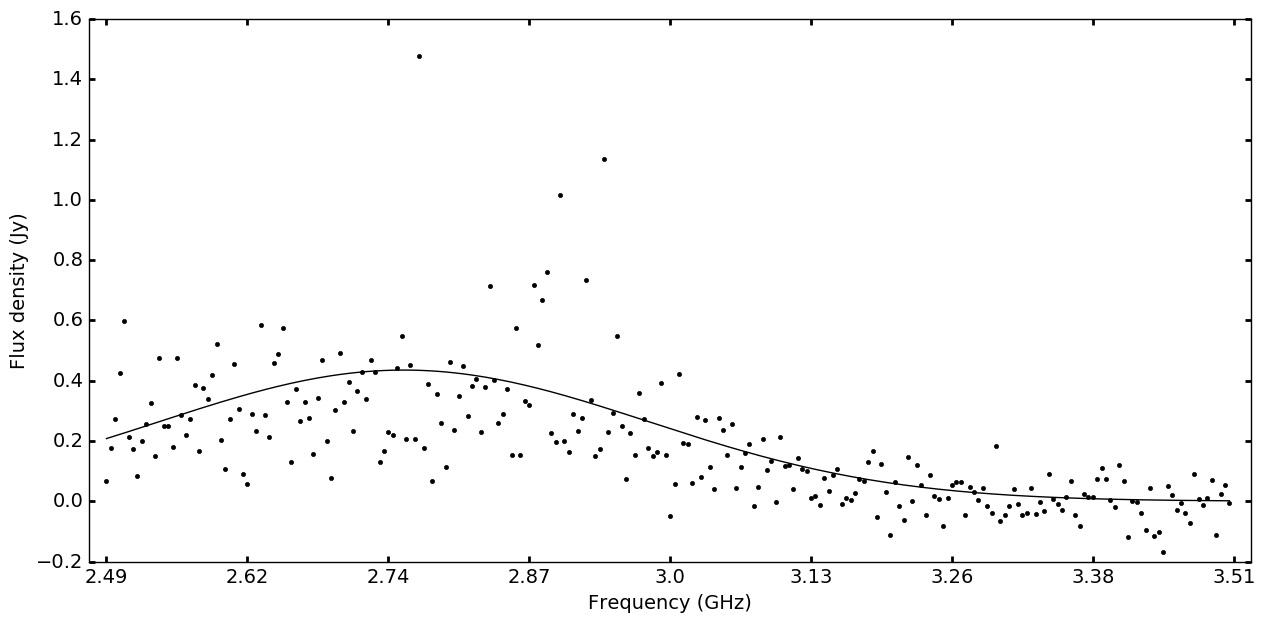
\includegraphics[width=0.33\columnwidth]{spec_57643.png}
  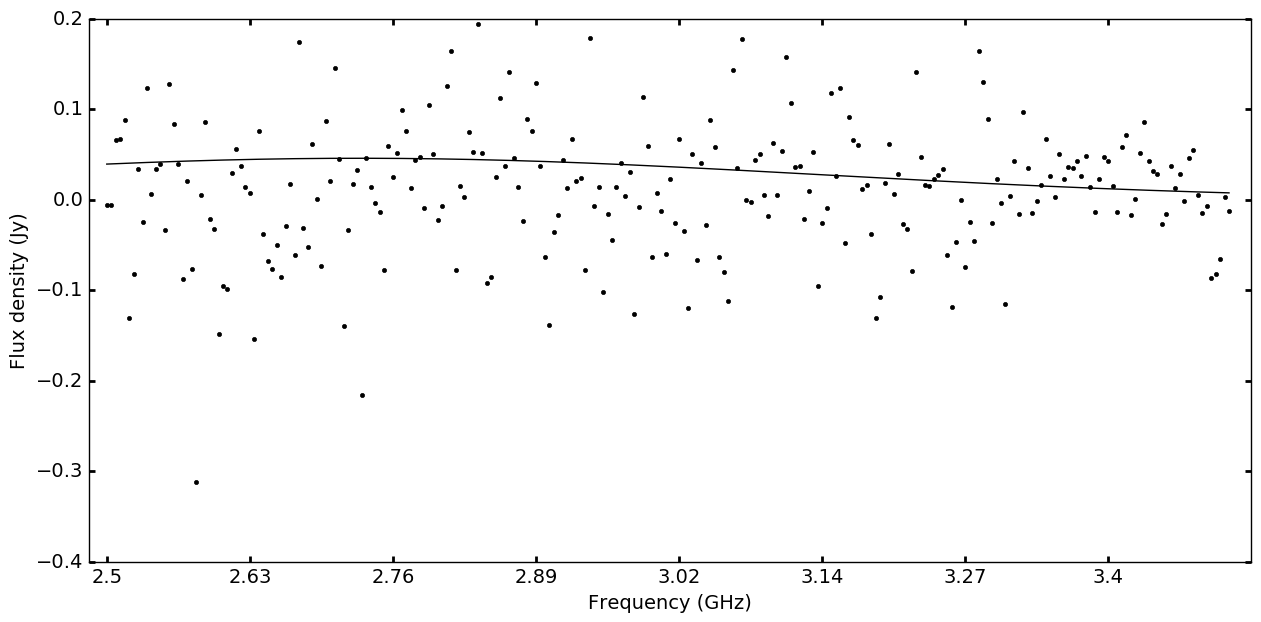
\includegraphics[width=0.33\columnwidth]{spec_57645.png}
 \end{minipage}

 \begin{minipage}{2\columnwidth}
  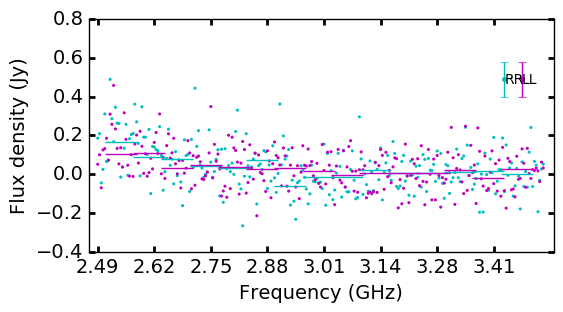
\includegraphics[width=0.33\columnwidth]{spec_57646.png}
  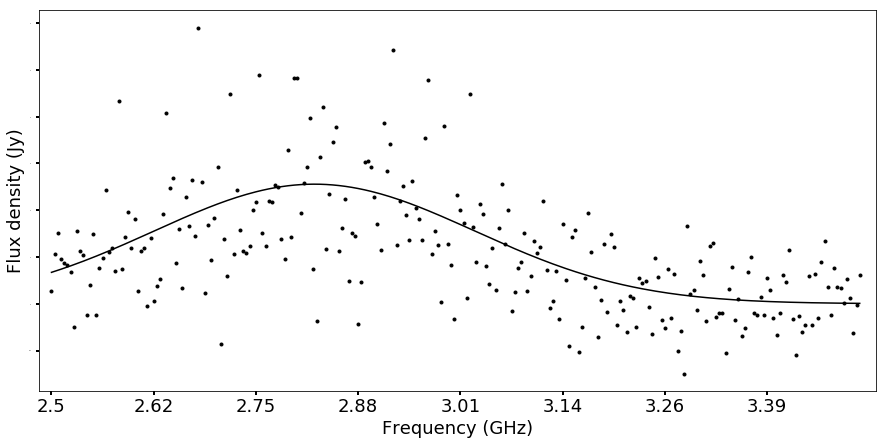
\includegraphics[width=0.33\columnwidth]{spec_57648.png}
  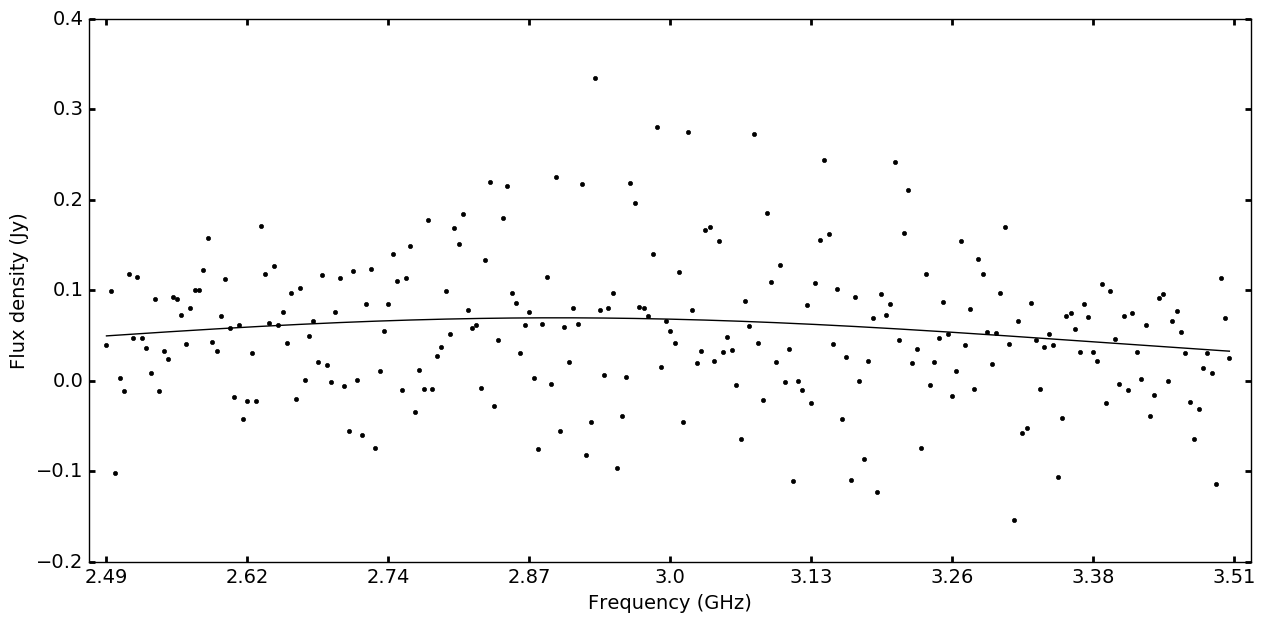
\includegraphics[width=0.33\columnwidth]{spec_57649.png}
 \end{minipage}
\caption{Spectra and best-fit model for nine bursts seen by the VLA from 2.5 to 3.5~GHz. Starting at the top left (moving right and then down), they correspond to bursts on MJDs 57623, 57633.68, 57633.70, 57638, 57643, 57645, 57646, 57648, and 57649. The solid line is a best-fit Gaussian model found through MCMC modeling. Note that bursts are detected in 5~ms images generated from dedispersed visibilities.
\label{fig:spec}}
\end{center}
\end{figure*}

This analysis differs from traditional analysis in that it simultaneously models the spectral and temporal evolution of the burst. Since the burst crosses many time-frequency pixel boundaries, the temporal modeling is sensitive to temporal properties smaller than the 5~ms integration time. Table \ref{tab:spec} shows that the typical burst width is measured as $2\pm1$~ms (95\% confidence interval); the brightest burst (57633.68) has a temporal width of $2.05\pm0.02$~ms. The burst arrival times are typically measured with a precision of 1~ms; the brightest burst arrival time is measured with a precision of $\sim50\mu$s. Note that these errors are only accurate to the degree that the model represents the data. One potential bias in the model is that we do not model scintillation effects.

**how does interchannel DM smearing compare to measured width?**

\begin{figure*}[htb]
\begin{center}
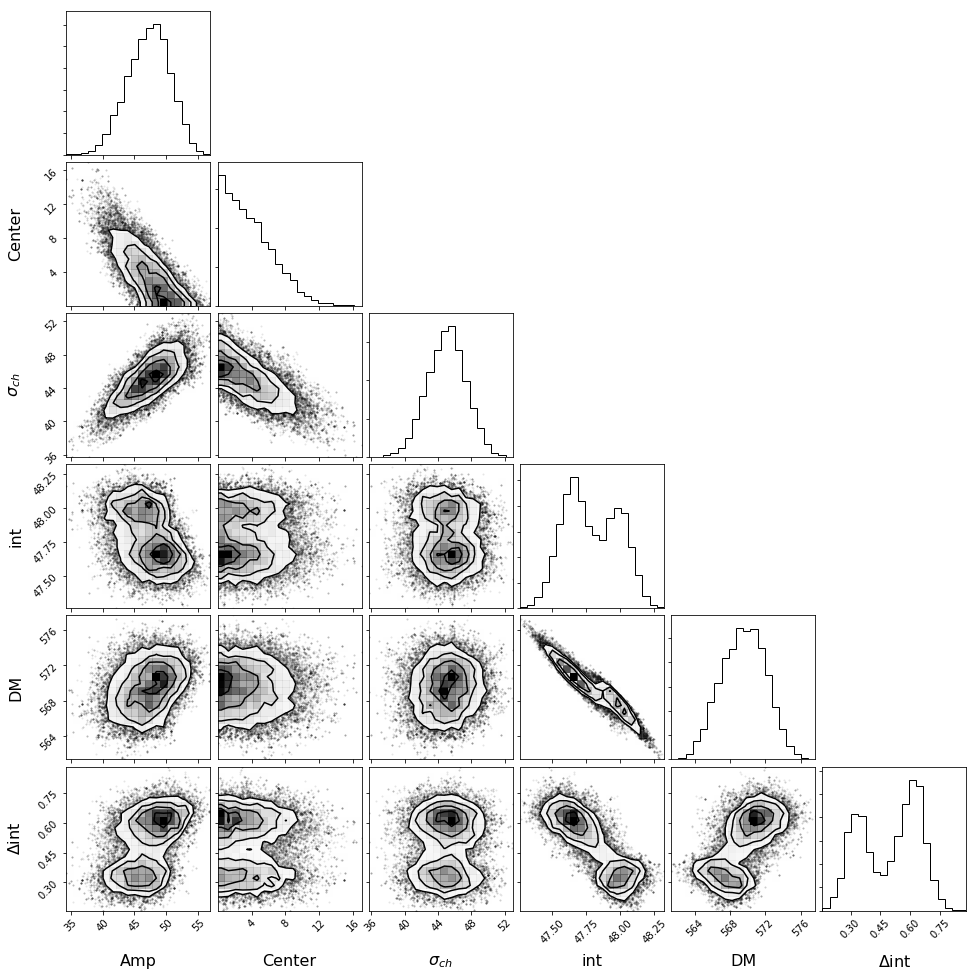
\includegraphics[width=2\columnwidth]{corner57646}
\caption{A scatterplot matrix that shows the correlation of every pair of parameters in the MCMC run for burst 57646. The equivalent plot for the other bursts show normally-distributed samples, but this burst shows significant structure in the samples.
\label{fig:corner}}
\end{center}
\end{figure*}

While most bursts are modeled with well-defined parameter probability distributions, one burst is an outlier. Figure \ref{fig:corner} shows the scatterplot matrix for the MCMC run on burst 57646 \citep{corner}. Two clusters of samples are identified for this burst: one narrow, low-DM and one wide, high-DM. The model seems to be too simple for this burst or that it can be decomposed into two bursts.

\subsubsection{Dispersion}

The initial VLA detections were made with a matched-filter approach that allowed inter-DM sensitivity losses up to roughly 10\% \citep[$\Delta \rm{DM}=10\ \rm{pc}\ \rm{cm}^{-3}$][]{2003ApJ...596.1142C}. 
%In optimizing detection significance over a fine DM grid, we find optimal DM values range from 552 to 572 pc cm$^{-3}$. However, the uncertainty in the peak DM measurement is defined by the signal-to-noise of the burst and how this changes with DM.
The MCMC modeling is more sophsticated in that it considers a wider range of parameters and models both data and observing effects (frequency-time pixel boundaries) simultaneously.

The top panel of Figure \ref{fig:dmmodel} shows the 95\% confidence intervals on the DM for all nine VLA bursts as a function of burst time. The burst DMs are not consistent with any single value and tend to be larger than the long-term average of 560.5 pc cm$^{-3}$. The range and variance in DM observed by the VLA is similar to that reported for Arecibo observations of \frb\ in \citet{2016arXiv160308880S}. As noted before, this is consistent with the idea that the DM measured at low temporal resolution (e.g., by the VLA or by single-dish observatories without coherent dedispersion) is determined by extrinsic (an electron column) dispersion and some spectral structure that changes between bursts. The VLA data demonstrate that the burst-dependent DM effect is visible at frequencies near 3~GHz. Assuming a ``true'' DM of 560.5 pc cm$^{-3}$, the excess DM can be thought of as a frequency-dependent delay that varies between bursts with a delay rate up to 2~ms GHz$^{-1}$ or an effective DM of $\sim5$~pc cm$^{-3}$.

The bottom panel of Figure \ref{fig:dmmodel} compares the DM to the modeled temporal width of the bursts. There is a weak correlation between burst width and apparent DM. A change in width of $\sim1$~ms correlates with a change in apparent DM of approximately $5$~pc cm$^{-3}$.

\begin{figure}[htb]
\begin{center}
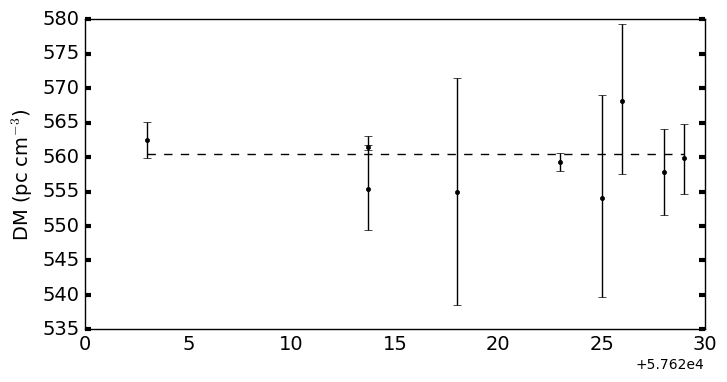
\includegraphics[width=\columnwidth]{dmmodel}

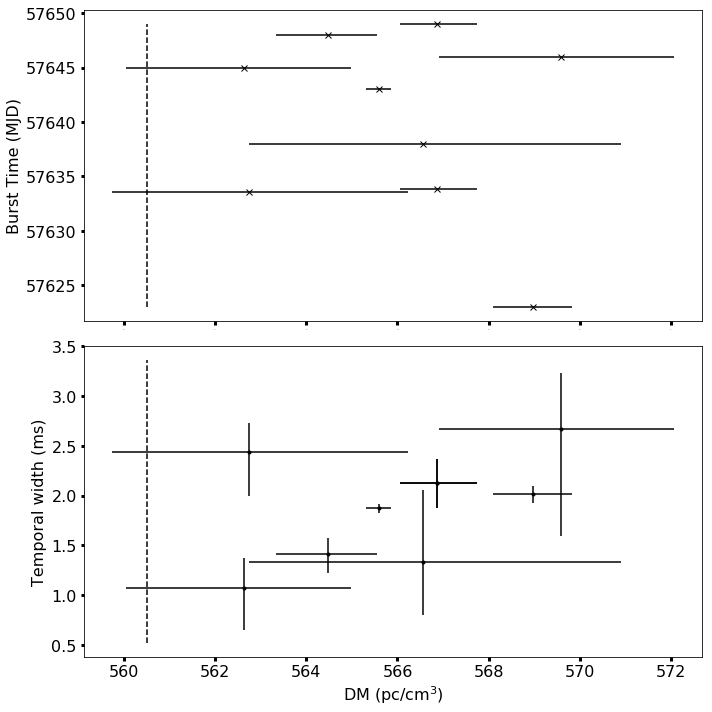
\includegraphics[width=\columnwidth]{burst_dmdt}

\caption{(Top) DM as a function of time for nine 3~GHz bursts detected by the VLA. The 95\% confidence interval on DM is shown with a bar and the dahsed line shows the best-fit DM$=560.5$\ pc cm$^{-3}$ inferred for Arecibo observations at 1.4~GHz. (Bottom) Burst DM versus temporal width for all nine VLA bursts.
\label{fig:dmmodel}}
\end{center}
\end{figure}

\subsection{Temporal Statistics}
\label{sec:temp}

The burst rate for \frb\ varied dramatically throughout the 2016 observing campaign (Figure \ref{fig:sched}). In the early-2016 campaign, we observed for 30 hours at S-band and no bursts were detected. In the late-2016 observing campaign, we observed for 27 hours at S-band an detected nine bursts. Overall, the data quality is uniform and high, so the inhomogeneous burst distribution shows that the burst detection probability was not stationary. Assuming that the burst detection probability follows a Poisson distribution, the nondetection in the first half of S-band limits the FRB rate to $\rm{R}<0.1$\ hour$^{-1}$\ (95\% confidence limit). The S-band burst rate was much higher during the late-2016 campaign, $\rm{R}=0.3\pm0.1$\ hour$^{-1}$.

\subsection{Energy and Brightness Distribution}
\label{sec:disn}

Knowing the source distance, we calculate the burst energy by integrating flux in time and frequency (Table \ref{tab:spec}). Some VLA burst spectra seem to be contained by the 2.5 to 3.5~GHz band and most of them seem to have Gaussian envelopes that are well modeled by the emission within that band. Assuming that the Gaussian shape defines the emission window, the mean S-band flux density can be converted to a total energy with no further assumptions about their spectral properties.

Figure \ref{fig:ed} shows the \frb\ burst energy cumulative distribution as seen by the VLA and calculated from prior observations by Arecibo and the GBT \citep{2016Natur.531..202S,2016arXiv160308880S}. The latter two energy distributions are scaled from the fluence by assuming that all burst energy is included by the observation. This likely underestimates the burst energy for some bursts by a factor of a few, but should not affect the slope of the distribution. The Arecibo and GBT energies were scaled by factors of {\color{red} 2 and 1 (anyone?)}, respectively, to correct for the sensitivity loss due to the primary beam.

Broadly, the range of energies shown in Figure \ref{fig:ed} is defined by the sensitivity of the telescope and the duration of the observing campaign. The VLA distribution shown represents the 27-hour, late-2016 campaign, which is longer than the single-dish campaigns presented here. However, since the VLA observations have a relatively coarse time resolution, it is not as sensitive as Arecibo and the GBT, so no bursts were detected weaker than $3\times10^{38}$~erg. The rate upper limit (95\% confidence) from the early-2016 VLA campaign shows that even identical observing campaigns have different detection rates.

We modeled the differential energy distribution, $dN/d\log{E}$, using a Poisson probability distribution with a rate function $\lambda = A E^{\alpha}$. Rather than trying to estimate a completeness limit for each energy distribution, we assume an effective detection limit of 0.9 times the weakest burst detected; the best-fit slope is weakly dependent on this, but general conclusions are robust. We directly sampled the likelihood distribution to estimate a best slope of $\alpha_{\rm{VLA}}=-0.7^{+0.3}_{-0.4}$, $\alpha_{\rm{AO}}=-0.8^{+0.3}_{-0.5}$, and $\alpha_{\rm{GBT}}=-0.8^{+0.4}_{-0.5}$ (68\% confidence interval). Expressed as a powerlaw function in $dN/dE$, the slope index is approximately --1.7. 

\begin{figure}[htb]
\begin{center}
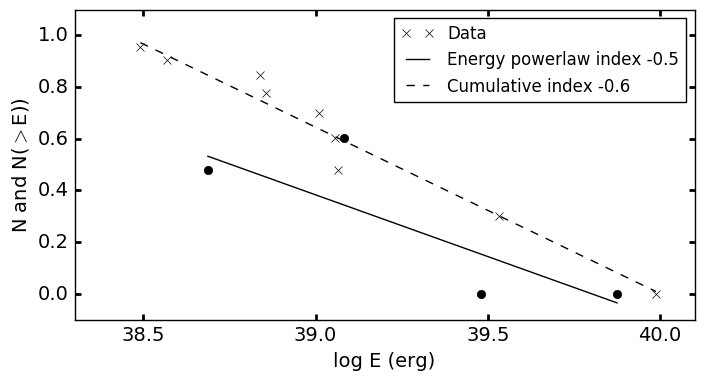
\includegraphics[width=\columnwidth]{energy_disn}
\caption{The cumulative burst energy distributions for the VLA, Arecibo, and GBT are shown with dots connected by solid, dashed, and dotted lines, respectively. The Arecibo distribution is derived from the 11 1.4~GHz bursts reported in \citet{2016Natur.531..202S} and the GBT distribution is derived from the 5 1.4~GHz bursts reported in \citet{2016arXiv160308880S}. An upper limit from the VLA nondetection in early 2016 is shown as a triangle. \label{fig:ed}}
\end{center}
\end{figure}

\section{discussion}
\label{sec:disc}
\subsection{Burst Spectra}

We present the first simultaneous detection of an FRB with multiple telescopes and over frequencies from 1.2 to 3.5~GHz. The Arecibo burst flux density is an order of magntude less than that seen by the VLA. At the same time, three other bursts from \frb\ had similar observing coverage but were not detected simultaneously. This is consistent with the spectral structure observed within the 3~GHz VLA band, which is typically limited to a Gaussian envelope with width of roughly 500~MHz. The center frequency of this envelope is a unique property of each burst and does not show an obvious pattern between bursts.

If \frb\ burst spectra are typical of the larger FRB population, then population models need to be generalized beyond the assumption of a spectral powerlaw. Most obviously, \frb\ implies that future multi-telescope searches for bursts are unlikely to simultaneously detect bursts in different bands. Second, since burst spectra have limited bands, the burst detection rate at one frequency may not represent that at another. That will require rate estimates for the FRB population to be made explicitly frequency-dependent. Finally, we note that the odds of detecting a burst will improve with bandwidth for bandwidths wider than their characteristic scale.

After correcting for barycentric and typical dispersion delays, the VLA/Arecibo burst spectrum shows a residual temporal drift. This drift can be interpreted as an excess DM of roughly 5 pc cm$^{-3}$. We also measure a burst-to-burst variation in DM within the whole sample of VLA 3~GHz bursts of a similar scale. This variation had been noted in earlier 1.4~GHz Arecibo observations of \frb\ \citep{2016arXiv160308880S}, but the VLA bursts demonstrate that this burst-specific DM is seen up to 3~GHz. The simultaneous VLA/Arecibo burst also shows that an individual burst's properties from 1.2 to 3.5~GHz are consistent with a single excess. 

These features are generally consistent with intrinsic burst properties described in \citet{WEIRD}. That work uses bright, coherently-dedispersed bursts to identify sub-bursts that preferentially drift to lower frequencies at later times. With high-resolution dynamic spectra, one can define a heuristic that distinguishes between a burst-specific dispersion-like effect and a more stable (``true'') dispersion. Since the sub-bursts tend to drift to lower frequencies, they systematically bias DM measurements made with low-resolution data (like the VLA and earlier Arecibo and GBT obsrevaitons). Interestingly, our modeling of the VLA burst dynamic spectra show a weak correlation between larger apparent DM and pulse width. This could be a signature of blending of many unresovled sub-bursts in a single VLA burst spectrum.

The burst-specific DM structure could be intrinsic to the emission mechanism or induced during propagation. Radio waves can be modified in a variety of ways (e.g., scintillation, scattering) and the duration of the emission in the source frame is not known \citep{2016arXiv160505890C}. \citet{CORDES} describe a model where plasma lensing near the source of an FRB can magnify radio emission by orders of mangitude. That model argues that the simultaneous appearance of a burst from 1.2 to 3.5~GHz requires a lens with the focal frequency be $\gtrsim 3.5$~GHz. This gives a constraint on the combination 
$$\frac{\rm DM_0}{a_{\rm AU}^2} \frac{d_{sl}d_{lo}/d_{so}}{1\, \rm kpc} \gtrsim (3.5 / 39.1)^2$$
where $DM_0$, $a$, and $d_*$\ are the electron column density of the lens, size of the lens, and lensing distances, respectively. A lens placed at $d_{sl}\approx1$~kpc is consistent with typical properties of the interstellar medium. Lenses that are influenced by the source would be much nearer to the source $d_{\sl} \ll 1$~kpc, requiring large values of $\frac{\rm DM_0}{a_{\rm AU}^2}$.

\subsection{Energy and Flux Distribution}

The refined analysis shows that \frb\ has even higher isotropic energies than previously reported, reaching energies $E_{\rm{max}}\approx10^{40}$\ erg. \frb\ has isotropic energies orders of magnitude higher than the strongest Crab pulsar pulses ($\sim10^{35}$~erg) and comparable brightness temperatures \citep[$T_b^{\rm{Crab}}\sim10^{41}$~K versus $T_b^{\rm{FRB 121102}}\sim10^{38}$~K;][]{2003Natur.422..141H,2014PhRvD..89j3009K}. 
%While this emission is coherent and strongly beamed \citep{2016Natur.531..202S, WEIRD}, the energy scale is still larger than any known Galactic radio transient and requires either a new process or dramatic scaling of known emission processes \citep{2016MNRAS.462..941L, 2016MNRAS.457..232C}.

In \S \ref{sec:disn} we compare the energy distribution of the 9 VLA bursts to those reported earlier by Arecibo and the GBT. All three energy distributions can be characterized as a powerlaw in $dN/dE$ with slope $\sim-1.7$. This slope is seen even though the burst rate varies by almost an order of magnitude between observations and frequencies cover both 1.4 and 3~GHz bands. This suggests that the slope is related to the underlying physical process, rather than the state at any given time. The value of the energy distribution slope is similar to that observed in gamma-ray fluence of bursts from soft-gamma repeaters \citep{2000ApJ...532L.121G, 2011ApJ...739...94S}. This similarity has been used to argue that bursts are driven by self-regulated critical phenomena \citep[slope$=-5/3$;][]{2011SoPh..274...99A}.

While the surprising brightness of new FRB discoveries was once seen as a cause for concern (i.e., a sign of terrestrial interference), we may be able to use this to infer properties of the overall population \citep{2007Sci...318..777L, 2016arXiv161105758R}. When modeling the flux distribution as a powerlaw, an isotropic distribution of sources will have a powerlaw index, $\alpha$, of --1.5 \citep[the ``Euclidean distribution'';][]{2016MNRAS.462..941L}. Prior to the measurement of the first GRB redshift, deviations from the Euclidean distribution were used to infer their cosmological distribution \citep[e.g., the $V/V_{\rm{max}}$\ test;][]{1992ApJ...388L..45M, 1995ApJ...453...25F}. Multiple studies have suggested that FRBs have a sub-Euclidean flux distribution \citep[$-0.5<\alpha<-0.9$;][]{2016ApJ...830...75V, 2016arXiv160206099L, 2016arXiv161100458L}. Others have noted that the flux distribution is not well modeled as a powerlaw, such that $\alpha$\ is effectively sensitivity (and telescope) dependent \citep{2016MNRAS.461..984O, 2017arXiv170208040C}.

We now know that \frb\ is detectable with the VLA out to $z=0.7$, which suggests that cosmological effects are even more important for understanding properites of the FRB population. \citet{2017arXiv170208040C} demonstrate how redshift space distortions, time dilation, and spectral index (``k-correction'') effects can flatten the flux distribution. To this complex scene, we add the fact that \frb\ burst spectra are not defined by a spectral index, which suggests that k-corrections are likely to be very difficult to calculate in practice. Rather than using wide band burst spectra to measure a single spectral index, we now must measure the burst rate as a function of frequency. These need to be measured at similar times to insure they represent a similar state of activitity of the FRB.

If we assume \frb\ is representative of the FRB population, we can estimate this frequency-dependent burst rate. The VLA and Arecibo observed intensively in a coordinated fashion during the late-2016 campaign. A complete search for bursts from the Arecibo is ongoing, but early results suggest that the burst rate at a fixed energy is much higher at 1.4~GHz than at 3~GHz. This suggests that high-redshift FRBs will have an apparently lower rate that flattens the $dN/dF$\ distribution in a manner similar to a k-correction. We can only infer the presence of this effect for observations near 1.4~GHz, since we have no estimate of the \frb\ burst rate outside the frequency range from 1.4 to 3~GHz. Propagation effects suggest that the rate will be lower at sub-GHz frequencies \citep{2017MNRAS.465.2286R}. If so, the tension between constraints on $\alpha$\ near 800~MHz and 1.4~GHz may be resolved by a frequency-dependent FRB rate that peaks near 1.4~GHz.

%While the \frb\ burst energy distribution is consistent with the overall FRB population, this simulation ignores many observational biases (scattering, observing coverage) and the effects of galaxy evolution, which is likely significant over the range of redshifts to which \frb\ is detectable \citep[e.g.,][]{2010ApJ...709..644I}. The burst energies are estimated from observations from 2.5 to 3.5~GHz, which may be a biased selection of all bursts or may not include all burst emission. If the simulation is revealing a connection between \frb\ and the broader FRB population, it does not explain the physical mechanism that drives it. The burst energy distribution of the population could be dominated by intrinsic or extrinsic effects \citep{2015MNRAS.451.3278M,2016Natur.531..202S,CORDES}. More FRB detections will improve the quality of this inference as sample variance drops, while more burst detetions from \frb\ will improve the measurement of the intrinsic energy distribution.

\subsection{Repetition}

The chance of detecting a burst with the VLA changes substantially on day--month timescales. A major outstanding question is whether this time-variable rate is driven by an intrinsic process \citep{2016ApJ...826..226K} or extrinsic (propagation) effects \citep{CORDES}. However, the temporal distribution of VLA detections alone shows that \frb\ has significant correlation on short timescales. That is, detecting a burst predicts you are more likely to find another burst soon thereafter and not detecting a burst predicts you will likey not detect another burst soon thereafter. While this is sometimes referred to as a ``red spectrum'' \citep{2016MNRAS.458L..89C}, the observations presented here are only sensitive to timescales of days (time between observations) and months (time between campaigns). 

If this statistical property describes other FRBs, it weakens previous constraints on repetition \citep{2015MNRAS.454..457P,2015ApJ...807...16L}. It is possible that other FRBs have repeating bursts, but calculating a limit requires knowing their temporal correlation function. Wide, shallow surveys are the preferred strategy for blind detection of FRBs. Also, since ``bursts predict bursts'', many short observations are more likely to blindly detect an FRB than a single long observation of the same total length. 

\subsection{Revised Volumetric Rate}

**correct for time dilation?**

%The calculation of a volumetric rate has been used to study classes of optical and high-energy transient \citep{2006ARA&A..44..507W}. 
\citet{2013Sci...341...53T} estimated an isotropic FRB rate of $10^{-3}$\ galaxy$^{-1}$\ yr$^{-1}$ by calculating the number of Milky Way-type galaxies out to a distance implied by assming all extragalactic DM originates in the IGM \citep[$z\approx0.9$\ for $DM\approx z\times900 \rm{pc}\ \rm{cm}^{-3}$;][]{2003ApJ...598L..79I,2004MNRAS.348..999I}. This rate is high \citep[comparable to the rate of core-collapse supernovae;][]{2006Natur.439...45D}, which has been used to argue that FRBs are likely not associated with other classes of transient, such as LGRBs or rarer SNe \citep{2006ARA&A..44..507W}. This challenges models for FRBs based on magnetars or young, fast pulsars, which are believed to power these rarer subclasses of optical/gamma-ray transient. However, since the FRB rate estimate depends on the telescope sensitivity, it is not appropriate to compare to other estimates based on source counts.

Here, we reevaluate the FRB volumetric rate by assuming \frb\ is a prototype of the class. First, we recast the estimate as volumetric rate of FRB sources by including beaming and repetition effects. The volumetric source rate is $R_{\rm{FRB}} = R_p /(N_r \Omega_b V (z))$, where $R_p$\ is the projected FRB rate, $N_r$\ is the number of bursts per source, $\Omega_b$\ is the beaming fraction, and $V(z)$\ is the volume out to redshift $z$. The newest estimates of the projected FRB rate are lower by a factor of 5 \citep[$2\times10^3\ \rm{sky}^{-1} \rm{day}^{-1}$\ at high Galactic latitudes and flux densities brighter than 1~Jy~ms; ][]{2016arXiv161100458L, 2016MNRAS.460L..30C, 2016MNRAS.455.2207R}. 

\frb\ has an absolute energy scale that can be used to convert the observation-dependent fluence limit into a characteristic FRB distance. At the typical Parkes survey parameters \citep[e.g.,][]{2016MNRAS.460L..30C}, a fluence limit of 1~Jy~ms is detectable at $z\approx1$. The distance inferred from the largest DMs observed \citep[$\sim1500$\ pc cm$^{-3}$;][]{2016MNRAS.460L..30C} is somewhat higher, but that likely overestimates distance since DM will have significant contributions from the host galaxy and intervening galaxies \citep{OPT, 2014ApJ...780L..33M}.
%For reference, we note that cosmic star formation rate peaks between redshift of 2 and 3\citep{2014ARA&A..52..415M}.

Using an assumed horizon redshift of 1, we estimate a rate of $R_{\rm{FRB}} \approx 5\times10^{-5} N_r^{-1} (0.1/\Omega_b)$\ Mpc$^{-3}$\ yr$^{-1}$. The narrow burst spectral structure seen for \frb\ implies that observations have undercounted the rate by a factor of a few by ignoring bursts outside the band. There is also relatively little constraint on the beaming factor \citep[$\sim0.1$ for pulsars;][]{1998MNRAS.298..625T}. Finally, we note that this estimate assumes that propagation effects do not significantly affect the detectability of FRBs, although scintillation and scattering likely play significant roles \citep{2015MNRAS.451.3278M, CORDES}.

Despite its many assumptions, this is the first volumetric rate appropriate for comparison to rates used for other classes of transient. The LGRB and SLSN-I rates are $10^{-7}$\ and $10^{-8}$\ Mpc$^{-3}$\ yr$^{-1}$, respectively \citep{2007ApJ...657L..73G,2012Sci...337..927G}. Comparing the FRB rate to these rates implies that FRB-emitting sources can be generated in LGRBs and SLSN-I if FRBs repeat $5\times10^2$\ and $5\times10^3$, respectively (assuming burst energies of $10^{40}$\ erg). \citet{2017arXiv170102370M} use the young magnetar model for FRBs to calculate the maximum number of bursts that can be powered its magnetic field as $\approx300$. Assuming this model for FRBs, LGRBs, and SLSN-I, the rate comparison suggests that the LGRB rate is most consistent with the FRB rate, although it is entirely possible that there are multiple channels to produce FRB-generating magnetars.

%\subsection{Naming Convention}
%The consistency of \frb\ properties (e.g., energy distribution) with the overall population suggests other FRBs likely repeat. If so, the current naming convention for FRBs (analogous to cataclysmic supernovae), will likely become uninformative, especially as large FRB survey projects come online \citep{2014SPIE.9145E..22B}. If all FRBs repeat, then a more useful convention would be based on coordinates. However, there are already two FRBs that have consistent celestial positions and different DMs. Therefore, we suggest an FRB naming convention as Jhhmm+ddDMmmmm.

\section{Conclusions}

The recent precision localization of \frb\ has helped identify a host galaxy, measure its distance, and establish it as a member of a truly new class of astrophysical source. With its cosmological distance firmly established, \frb\ now serves as a new kind of standard by which FRBs are defined. That fact, combined with an abundance of data collected during its high activity state, allows us to apply this source to more general questions about the FRB population.

We presented the first multi-telescope detection (Arecibo and VLA) of an FRB. By detecting this burst from 1.2 to 4.5~GHz, we have demonstrated that some bursts have broad spectral structure. However, the energy of that burst was dominated by the VLA 3~GHz observing band and three other VLA bursts are undetected by Arecibo. That demonstrates the burst spectra cannot be characterized by a spectral index. Independently, we modelled dynamic spectra within the VLA 3~GHz band and show that most burst can be characterized by a Gaussian envelope of width $\sim500$\ MHz. This modeling also shows that the apparent DM changes from burst to burst. DM values are biased above the long-term average, which argues that bursts have intrinsic spectral structure that mimics DM. This confirms analysis of high-resolution Arecibo dynamic spectra and extends this phenomenology to the 3~GHz band.

With a characteristic width of a spectrum, we can estimate total (apparent) radio energy per bust. The cumulative energy distribution is characterized by a powerlaw in $dN/dE$ with slope of $\sim-1.7$. The amplitude of this powerlaw changes significantly between observational campaigns. The stochastic nature of the burst rate suggestts that past constraints on FRB repetition are weaker than previously inferred. The relatively narrow spectral structure, flat energy distribution, and variable burst rate of \frb\ suggests that repeated observations, wide bandwidth, and large instantaneous field of view all improve the chance of making new FRB detections.

Assuming that \frb\ is reprentative of the FRB population, its burst energy distribution makes it possible to calculate the first volumetric FRB rate that does not depend on telescope sensitivity. We estimate a volumetric rate of $R_{\rm{FRB}} \approx 5\times10^{-5} (0.1/\Omega_b)$\ Mpc$^{-3}$\ yr$^{-1}$, which is appropriate for \frb-like energies of $10^{40}$\ erg that are detectable out to $z=1$. This rate is broadly consistent with models of FRBs from young magnetars or fast pulsars if the typical FRB repeats on the order of $10^3$\ times in its life.

New, arcsecond-scale localizations will be critical to refining the picture presented here and constraining models of FRB origin. \frb\ was localized within hours by a prototype version of \rf\ and an expanded \rf\ system is now under construction. This platform will search a TB/hour data stream in real time in parallel with ongoing VLA observations, potentially detecting and localizing multiple FRBs per year.

\bibliographystyle{apj}

\section*{Acknowledgements}
% observatories
The National Radio Astronomy Observatory is a facility of the National Science Foundation operated under cooperative agreement by Associated Universities, Inc..
% systems
This research made use of Astropy, a community-developed core Python package for Astronomy (Astropy Collaboration, 2013).
%individuals
CJL is supported by the University of California Office of the President under Lab Fees Research Program Award 237863 and NSF award 1611606. MAM is supported by NSF award \#1458952. KPM's research is supported by the Oxford Centre for Astrophysical Surveys which is funded through the Hintze Family Charitable Foundation. AS gratefully acknowledges support from the European Research Council under grant ERC-2012- StG-307215 LODESTONE. The AMI-LA telescope gratefully acknowledges support from the European Research Council under grant ERC-2012- StG-307215 LODESTONE, the UK Science and Technology Facilities Council (STFC) and the University of Cambridge.

We thank Liam Connor for useful feedback and the VLA staff for their support of \rf\ development. We acknowledge partial support from the Research Corporation for Scientific Advancement (RCSA) for participation in the meeting Fast Radio Bursts: New Probes of Fundamental Physics and Cosmology at the Aspen Center for Physics (February 12-17, 2017).

\bibliography{fasttrants.bib}

\end{document}

